    \begin{figure} [H]
    \begin{centering}
    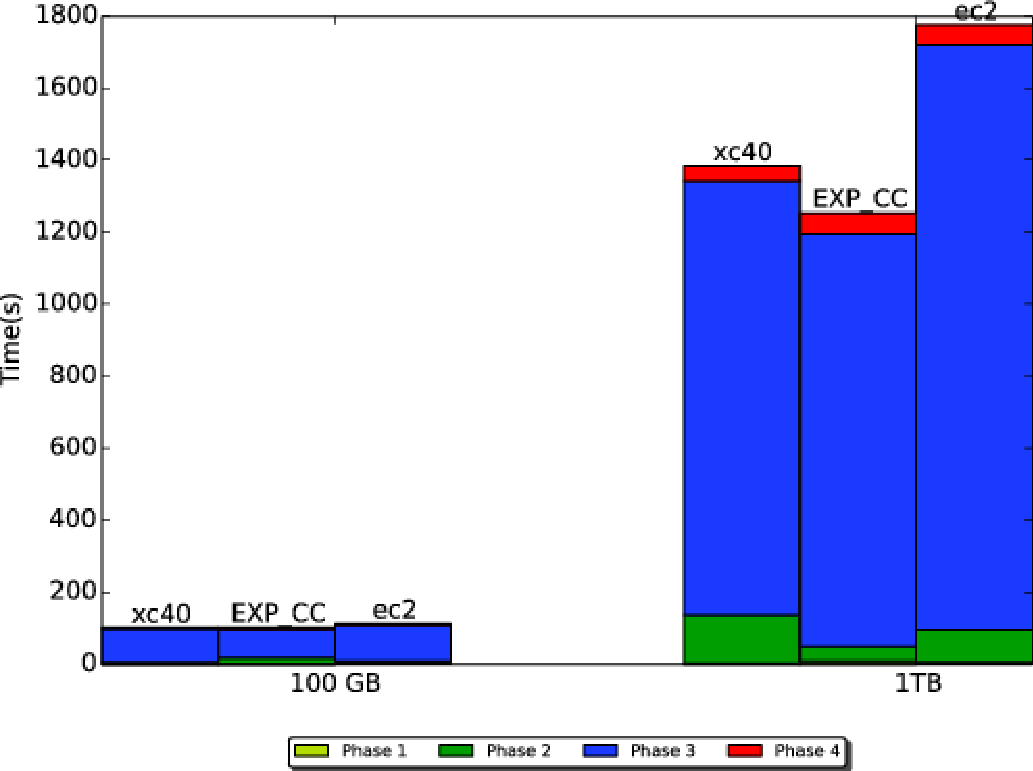
\includegraphics[scale=0.4]{images/CX_Size_Scaling_Rank_32_Partitions_default.pdf}
    \end{centering}
    \caption{ Run times for the various stages of computation for CX for two different dataset sizes for the three platforms using rank 32 and default partitioning for the given platform}
    \label{fig:h2hrank32} 
    \end{figure}
    
    \begin{table*}
    \begin{center}
    \begin{tabular}{| l | c | c | c | c | c | c | c |}
    \toprule
    \textbf{Platform} & \textbf{Rank} & \textbf{Total} & \textbf{Load} & \textbf{Time Per} & \textbf{Average} & \textbf{Average} & \textbf{Average} \\
                               & & \textbf{Runtime} & \textbf{Time} & \textbf{Iteration} & \textbf{Local} & \textbf{Aggregation} & \textbf{Network} \\
                               & & & & & \textbf{Task} & \textbf{Task} & \textbf{Wait} \\
    \midrule
    Amazon EC2 r3.8xlarge & 16 & 24.0 min & 1.53 min & 2.69 min & 4.4 sec & 27.1 sec & 21.7 sec \\
    \midrule
    Cray XC40 & 16 & 23.1 min& 2.32 min & 2.09 min &  3.5 sec & 6.8 sec & 1.1 sec \\
    \midrule
    Experimental Cray cluster & 16 & 15.2 min & 0.88 min & 1.54 min &  2.8 sec & 9.9 sec & 2.7 sec \\
    \midrule
    Amazon EC2 r3.8xlarge & 32 & 52.6 min& 1.57 min & 5.42 min &  8.7 sec & 60.1 sec & 48.7 sec \\
    \midrule
    Cray XC40 & 32 & 41.2 min & 2.28 min & 4.01 min &  7.5 sec & 25.0 sec & 15.4 sec \\
    \midrule
   Experimental Cray cluster & 32 & 35.8 min & 0.81 min & 3.82 min &  6.8 sec & 27.9 sec & 15.5 sec \\
   \bottomrule
    \end{tabular}
    \end{center}
    \caption{Total runtime for the 1 TB dataset, broken down into load time and per-iteration time. The per-iteration time is further broken down into the average time for each task of the local stage and each task of the aggregation stage.  We also show the average amount of time spent waiting for a network fetch, to illustrate the impact of the interconnect.}
    \label{tab:h2hres1TB}
    \end{table*}
    
Table~\ref{tab:h2hres1TB} shows the total runtime of CX for the 1 TB dataset on our three platforms.  The distributed Spark portion of the computation is also depicted visually in Figures~\ref{fig:h2hrank16} (rank 16) and~\ref{fig:h2hrank32} (rank 32).  All three platforms were able to successfully process the 1 TB dataset at rank 16 in under 25 minutes.  As the table and figures illustrate, most of the variation between the platforms occurred during the \texttt{MultiplyGramian} iterations.  Table~\ref{tab:hwspecs} shows the specifications of the three platforms. In this section, we explore how these difference relate to the performance of the matrix iterations.

Spark divides each iteration into two stages.  The first \emph{local} stage computes each row's contribution, sums the local results (the rows computed by the same worker node), and records these locally-aggregated results.  The second \emph{aggregation} stage combines all of the workers' locally-aggregated results using a tree-structured reduction.  Most of the variation between platforms occurs during the aggregation phase, where data from remote worker nodes is fetched and combined.  In Spark, all inter-node data exchange occurs via \emph{shuffle operations}.  In a shuffle, workers with data to send write the data to their local scratch space.  Once all data has been written, workers with data to retrieve from remote nodes request that data from the sender's block manager, which in turns retrieves if from the senders local scratch space, and sends it over the interconnect to the receiving node.

Examining our three platforms (Table~\ref{tab:hwspecs}), we notice two key hardware differences that impact shuffle operations.  First, both the EC2 nodes and the experimental Cray cluster nodes have fast SSD storage local to the compute nodes.  The Cray\textregistered~XC40\textsuperscript{\tiny\texttrademark} system~\cite{alverson2012cray,craycascadesc12}, on the other hand, has no local block storage.  Thus it must emulate local storage with a remote Lustre filesystem.  The impacts of this can be somewhat mitigated, however, by leaving sufficient memory to store some of the scratch data in local RAM disk, and to locally cache some of the remote writes to Lustre.\footnote{This is an ideal usage of caching, since Spark assumes the scratch space is only locally accessible; thus we are guaranteed that the only node that reads a scratch file will be the same node that wrote it.}  Second, the Cray XC40 and the experimental Cray cluster both communicate over the HPC-optimized Cray Aries 
interconnect~\cite{alverson2012cray,craycascadesc12}, while the EC2 nodes use 10 Gigabit Ethernet.  

   \begin{figure} [H]
    \begin{centering}
    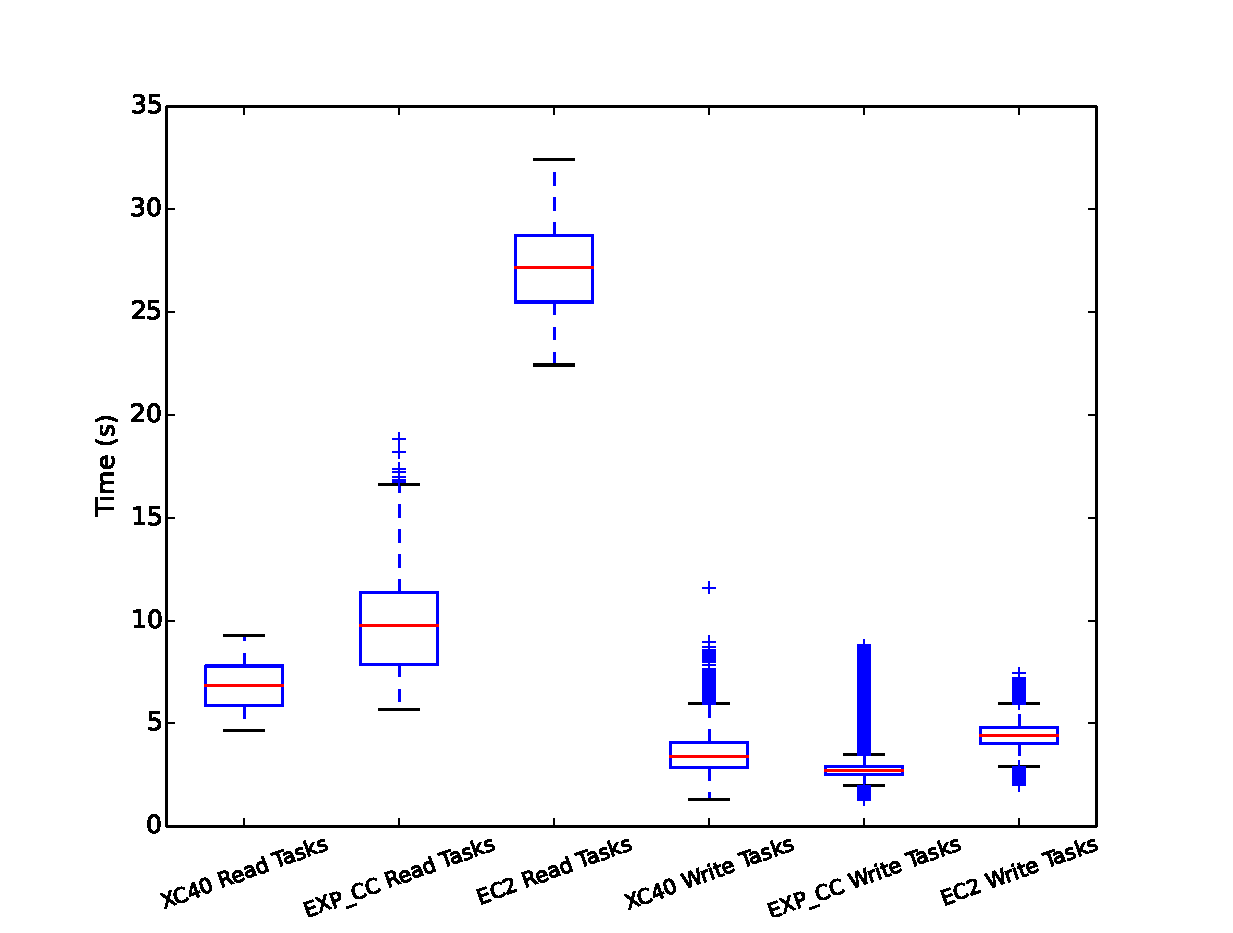
\includegraphics[scale=0.4]{images/boxplot_read_write_task_new_Rank_16_1T_default_partitions.eps}
    \end{centering}
    \caption{A box and whisker plot of the distribution of local (write) and aggregation (read) task times on our three platforms for the 1TB dataset with rank 16.  The boxes represent the 25th through 75th percentiles, and the lines in the middle of the boxes represent the medians.  The whiskers are set at 1.5 box widths outside the boxes, and the crosses are outliers (results outside the whiskers).}
    \label{fig:rwtaskdist} 
    \end{figure}

We can see the impact of differing interconnect capabilities in the Average Network Wait column in Table~\ref{tab:h2hres1TB}.   These lower average network wait times explain why the two Cray platforms outperform the EC2 instance (with the experimental cluster achieving a speedup of roughly 1.5x over EC2).  

The XC40 is still slightly slower than the experimental Cray platform, however, in particular at rank 16.  This can be understood by looking at the distribution of local (write) task times in the box and whiskers plot in Figure~\ref{fig:rwtaskdist}.  We see that the XC40 local (write) tasks had a similar median time to the experimental cluster's local tasks, but a much wider distribution.  The large tail of slower "straggler" tasks is the result of some shuffle data going to the remote Lustre file system rather than being cached locally. We enabled Spark's optional speculative reexecution (\texttt{spark.speculation}) for the XC40 runs, and saw that some of these tasks were successfully speculatively executed on alternate nodes with more available OS cache, and in some case finished earlier.  This eliminated many of the straggler tasks and brought our performance closer to the experimental Cray cluster, but still did not match it (the results in Figures~\ref{fig:h2hrank16} and~\ref{fig:h2hrank32} and Table~\ref{tab:h2hres1TB} include this configuration optimization).  We discuss future directions for improving the performance on Spark on HPC systems in Section~\ref{sect:lessons}.
